\chapter{Grundlæggende}

\section{Hvad er en graf?}%
\label{sec:label}

Königsberg-problemet er ofte sagt til at være problemet der ``startede'' graf-teori. Beboerne af Königsberg i Preussen (i dag er dette \href{https://en.wikipedia.org/wiki/Kaliningrad}{Kaliningrad, Rusland}). Beboerne ville vide om det var muligt at gå over alle 7 broer blandt de to øer og land, og komme tilbage til hvor man startede. I Figur~\ref{fig:konigsberg} ses øerne, markeret henholdsvis $W$ og $Y$, de to landmasser, markeret $Z$ i syd og $X$ i nord, og de 7 broer i rød.\footnote{Billedet er opskaleret med AI, da der ikke var nogen billeder i en opløsning, hvor man kunne se noget.} Det kan være svært at se fra billedet, og det er derfor nemmere at abstrahere til en graf, som kan ses i Figur~\ref{fig:konigsberggraf}. I denne graf er hver af kanterne en bro, og knuderne er land. Man kan her se hvordan der er brug for et lige antal broer for at kunne starte et sted, krydse alle broerne, og så komme tilbage til det originale sted.


\begin{figure}[h!]
  \centering
  \begin{minipage}{0.45\textwidth}
    \centering
    \includegraphics[width=\textwidth]{figurer/Königsberg.jpg}
    \caption{\label{fig:konigsberg} Königsberg Broer}
  \end{minipage}
  \hfill
  \begin{minipage}{0.45\textwidth}
    \centering
    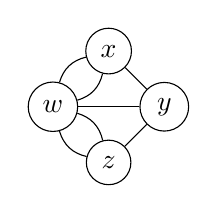
\begin{tikzpicture}[main/.style = {draw, circle}]
      \node[main] (w) {$w$};
      \node[main] (x) [above right of =w]{$x$};
      \node[main] (z) [below right of = w]{$z$};
      \node[main] (y) [above right of =z]{$y$};

      \draw (w) [bend right] to (x);
      \draw (x) [bend right] to (w);
      \draw (x) to (y);
      \draw (w) to (y);
      \draw (z) to (y);
      \draw (w) [bend right] to (z);
      \draw (z) [bend right] to (w);
    \end{tikzpicture}
    \caption{\label{fig:konigsberggraf} Graf til Königsberg Broer}
  \end{minipage}
\end{figure}

Vi vil nu definere hvad en \textit{graf} egentlig er.

\index{graf!definition}
\begin{definition}[Graf]
En \textbf{graf} $G$ er en triple indeholdende knudemængden $V(G)$, en mængde af kanter $E(G)$ og en relation som associerer hver kant til to knuder, kaldet endepunkter.
\end{definition}

Jeg har allerede brugt ordene ``knuder'' og ``kanter''. I Figur~\ref{fig:konigsberggraf} kan man se et eksempel på en graf, hvor knuderne er repræsenteret af cirkler med et ``navn'' (inde i cirklen) og en kant der går mellem. Dette er den mest normale måde at repræsentere en graf på. Mængden af kanter er $\{w,x,y,z\}$ og mængden af kanter er unavngivet. En anden måde at definere en graf på er ved at bruge en 2-tuple (også kaldet et par), hvor knuderne forbliver defineret på samme måde, men kanterne i stedet defineres som en mængde af par, hvor parrene er to knuder. Her ville vi kunne definere kanterne som den følgende mængde: $\{(w,x), (x,w), (w,z), (z,w), (w,y), (x,y), (z,y)\}$. West bruger også denne notation, dog uden at gøre det til par, i.e. bliver vores mængde til $\{wx, xw, wz, zw, wy, xy, zy\}$

\index{graf!løkke}
\index{graf!multiple kanter}
\index{graf!nabokanter}
\begin{definition}[Løkke]
En løkke er en kant hvis endepunkter er ens. Hvis et par af knuder har det samme par af endepunkter, kaldes de \textit{multiple kanter}. Når to kanter $u$ og $v$ er endepunkter af en kant er de \textit{naboer}\footnote{På engelsk siger man også at de to knuder er \textit{adjacent}.}. Vi skriver $u \leftrightarrow v$ til at mene ``$u$ og $v$ er nabokanter''.
\end{definition}

En graf er \textit{endelig} hvis mængden af kanter og knuder er endelige. Grafer i disse noter er endelige, undtagen hvis andet er sagt.

\index{graf!tom}
\begin{remark}
\textit{Den tomme graf} (engelsk: null graph) er grafen hvis mængder af kanter og knuder er tomme. Den bliver generelt ikke brugt, og skal derfor ikke haves i baghovedet når man læser teksten.
\end{remark}

\subsection{Grafer som Modeller}%
\label{subsec:grafersommodeller}

Vi kan bruge grafer til at modellere mange problemer. Før vi går videre til et eksempel, giver vi definitionen på komplementet af en graf:
\index{graf!komplement}
\begin{definition}[Komplement af en graf]
Komplementet $\overline{G}$ af en simpel graf $G$ er denne simple graf med knudemængden $V(G)$ defineret ved at $(u,v) \in E(\overline{G})$ hvis og kun hvis $(u,v) \in E(G)$.
\end{definition}

Vi kan nu se på et eksempel. Vi kan bruge grafer til at modellere om folk kender hinanden eller ej (ligeledes om deres forhold generelt: venner, fjender, bekendte, etc).


\begin{example}
  \label{ex:1.1.7}
Har alle mængder af seks personer 3 fælles bekendte eller 3 fælles fremmede? Vi kan modellere dette med grafer, ved den viden at bekendtskaber er fælles. Hver knude repræsenterer en person, og hver kant et bekendtskab. Dermed, hvis der er en kant mellem to knuder er disse personer bekendte.
\begin{figure}[H]
  \centering
  \begin{minipage}{0.45\textwidth}
    \centering
    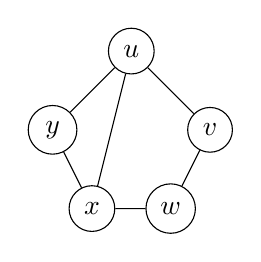
\begin{tikzpicture}[main/.style = {draw, circle}]
      \node[main] (u) at (0,0) {$u$};
      \node[main] (y) at (-1,-1) {$y$};
      \node[main] (x) at (-0.5,-2) {$x$};
      \node[main] (w) at (0.5,-2) {$w$};
      \node[main] (v) at (1,-1) {$v$};

      \draw (y) to (u)
      (u) to (v)
      (v) to (w)
      (w) to (x)
      (x) to (y)
      (u) to (x);

    \end{tikzpicture}
    \caption{\label{} Grafen $G$}
  \end{minipage}
  \hfill
  \begin{minipage}{0.45\textwidth}
    \centering
    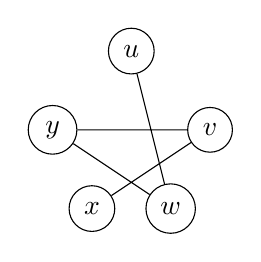
\begin{tikzpicture}[main/.style = {draw, circle}]
      \node[main] (u) at (0,0) {$u$};
      \node[main] (y) at (-1,-1) {$y$};
      \node[main] (x) at (-0.5,-2) {$x$};
      \node[main] (w) at (0.5,-2) {$w$};
      \node[main] (v) at (1,-1) {$v$};

      \draw (u) to (w)
      (w) to (y)
      (y) to (v)
      (v) to (x);

    \end{tikzpicture}
    \caption{Grafen $\overline{G}$}
  \end{minipage}
\end{figure}
  Her kan vi se at komplementet, giver de personer der er fremmede endnu.
\end{example}



\index{graf!klikke}
\index{graf!uafhængig mængde}
\begin{definition}[Klikke, uafhængig mængde]
En \textit{klikke} i en graf er en mængde af parvise naboknuder. En \textit{uafhængig mængde} (eller en stabil mængde) i en graf er en mængde af parvise knuder der \textbf{ikke} er naboer.
\end{definition}

Husk at to knuder er naboer når der er en kant imellem dem. Dermed kan du omformulere begge definition til at være følgende: En klikke er en delgraf hvor alle knuderne har kanter til alle andre knuder. En uafhængig graf er en delgraf hvor ingen af knuderne har kanter til nogen af de andre knuder.

I eksempel~\ref{ex:1.1.7} er $\{u,x,y\}$ en klikke af størrelse 3, og $\{u,w\}$ er en uafhængig mængde af størrelse 2. Under komplementet er disse omvendte, så $\{u,x,y\}$ er en uafhængig mængde, og $\{u,w\}$ er en klikke.

\index{graf!todelt}
\begin{definition}[Todelt Graf]
En graf $G$ er todelt (bipartite) hvis $V(G)$ er foreningsmængden af to disjunkte uafhængige mængder kaldet \textit{delte mængder} (partite sets) af $G$.
\end{definition}

\begin{example}
Hvis vi har $m$ jobs og $n$ personer, men ikke alle personer er kvalificeret til alle jobs, kan vi udfylde jobsne med kvalificeret personer? Vi kan modellere dette med en todelt graf, hvor jobs er en delgraf og personer er en anden. En person $p$ er nabo med job $j$ hvis $p$ er kvalificeret til $j$.
\begin{center}
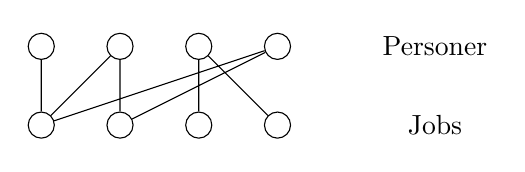
\begin{tikzpicture}[main/.style = {draw, circle}]
\node[main] (p1) at (0,1) {};
\node[main] (p2) at (1,1) {};
\node[main] (p3) at (2,1) {};
\node[main] (p4) at (3,1) {};
\node (personer) at (5,1) {Personer};
\node[main] (j1) at (0,0) {};
\node[main] (j2) at (1,0) {};
\node[main] (j3) at (2,0) {};
\node[main] (j4) at (3,0) {};
\node (jobs) at (5,0) {Jobs};

\draw (p1) to (j1)
(p2) to (j1)
(p2) to (j2)
(p3) to (j3)
(p3) to (j4)
(p4) to (j1)
(p4) to (j2);
\end{tikzpicture}
\end{center}
\end{example}

\index{graf!kromatisk tal}
\begin{definition}[Kromatisk Tal]
Det kromatiske tal af en graf $G$, skrevet $\chi(G)$ er minimumsantallet af farver nødvendige at give til knuder, således at naboknuder har forskellige farver.
\end{definition}

\index{graf!$k$-delelighed}
\begin{definition}[$k$-delelighed]
En graf $G$ er $k$-delelig hvis $V(G)$ kan udtrykkes som foreningsmængden af (muligvis tomme) uafhængige mængder.
\end{definition}

\begin{example}
Hvis vi har en mængde af komitéer, hvor nogle personer er i mere end en komité, og vi gerne vil planlægge tidspunktet for møder i disse komitéer, hvor mange forskellige tidspunkter skal vi bruge? Her er tidspunkterne farverne, så det minimum antal farver vi skal bruge, er også det minimum antal tidspunkter.
\end{example}


%%% Local Variables:
%%% mode: latex
%%% TeX-engine: xetex
%%% TeX-command-extra-options: "-shell-escape"
%%% TeX-master: "main"
%%% End:
